% Integrated from Sol; root edits follow in this file.
\section{Economic behavior across complete games}
\label{sec:sol-economic-results}

The economic trajectory runs from acquiring incomplete portfolios to developing income, financing shocks and receiving or losing estates. The cohort's winners are Sol in eight games, Gemini in seven, Opus in three and Grok in two. Figure~\ref{fig:cohort} shows why these totals are descriptive: Sol wins all four rotations of one seed block, while a different block is won from seat~2 by all four models. Shared raw dice do not supply matched economic opportunities or an independent ranking. The following results trace what agents actually acquired, financed and realized along these paths.

\begin{figure}[t]
\centering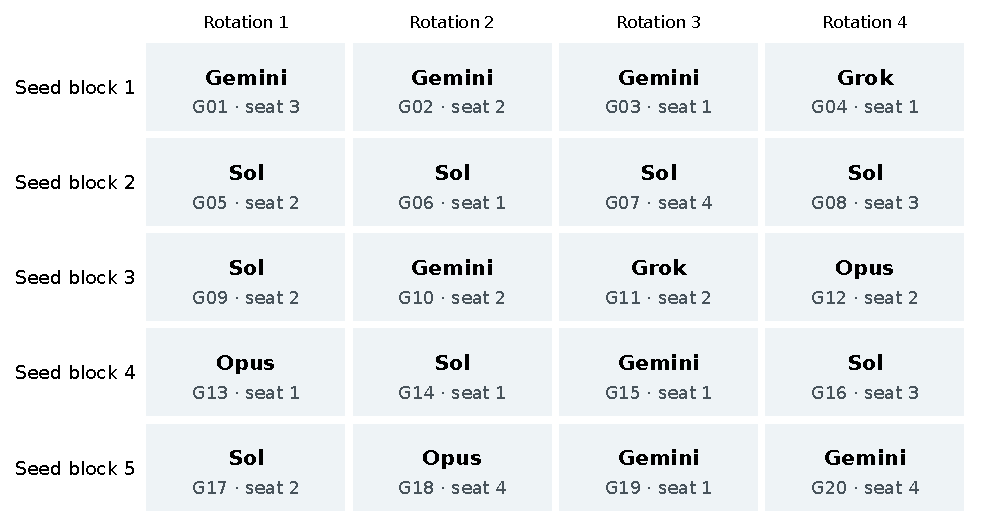
\includegraphics[width=\linewidth]{cohort.pdf}
\caption{Winner and seat in all twenty games. Each row shares an initial seed and contains four cyclic rotations. Outcomes are one realization per cell, not a repeated-trial reliability estimate. The two source fingerprints divide G1--4 from G5--20; their inspected diff does not change engine or prompt files.}
\label{fig:cohort}
\end{figure}

\subsection{Acquisition and bargaining create several routes to victory}

\begin{table}[t]
\centering\small
\begin{tabular}{lrrrrr}\toprule
Agent & Proposals & Proposing/eligible turns & Share & Intensity & Eligible decisions\\\midrule
Sol & 132 & 83/834 & 10.0\% & 1.59 & 1,133 \\
Gemini & 18 & 16/766 & 2.1\% & 1.12 & 1,001 \\
Opus & 240 & 160/660 & 24.2\% & 1.50 & 1,050 \\
Grok & 136 & 106/676 & 15.7\% & 1.28 & 897 \\
\bottomrule\end{tabular}
\caption{Negotiation initiation. Intensity is proposals per proposing turn. The final column records a different, action-dependent denominator; it is not an additional set of independent opportunities. Rounding uses two-decimal half-even display where applicable. All conditions in Table~\ref{tab:configurations} remain in these configured-system counts.}
\label{tab:negotiation}
\end{table}


Across the cohort, the event accounting records 475 direct, 72 auction, 207 trade and 397 inherited deed acquisitions. These are ownership transitions, including repeated acquisitions of the same deed. The distinct group-completion denominator contains 209 episodes: sixteen direct-purchase completions, nine auction completions, sixty-three trade completions and 121 inheritance completions. Sixty-nine inherited completions occur at game-ending bankruptcy and offer no subsequent opportunity. Counting all complete groups as productive achievements would therefore overstate what the surviving agent had occasion to use.

Negotiation varies substantially in activity and role. Sol proposes on 83 of 834 eligible own turns, Gemini on sixteen of 766, Opus on 160 of 660 and Grok on 106 of 676. Their proposal totals are 132, eighteen, 240 and 136, respectively. Gemini's low initiation coexists with twenty-six applied acceptances. These acceptances count the accepting actor, rather than both sides of a settlement. Recipient participation can therefore matter even when a participant seldom opens a thread. Conversely, repeated proposals can reflect an extended search for an acceptable exchange without producing a settlement.

The 113 settlements complete a color group for neither party in sixty cases, one party in forty-three, and both parties in ten. In forty-four settlements, the final offer's author differs from the original thread initiator. Bilateral reconstruction is necessary both for interpreting bargaining and for avoiding an attribution error in which the initiating agent receives credit for the other party's counteroffer. Group completion is one observable consequence. A transaction can also exchange railroad income, clear or mortgaged deeds, cash reserves and blocking positions. It can finance the seller's construction while giving the buyer a complete group. A completion count consequently cannot decide which side benefits, much less supply a welfare score.

Sol's G20 New York negotiation illustrates why a development budget must specify which existing assets it preserves. At d235, accepting the actual \$400 offer would leave \$97 after transfer interest. Tested spare mortgages, redemption and four orange houses leave \$41 while preserving brown hotels. Six houses are also reachable with \$91 left if Sol liquidates brown development. At d257, a diagnostic branch replacing Grok's actual rejection with acceptance of Sol's \$250 offer permits six orange houses with \$64 remaining while preserving the browns. Thus the six-house target is unavailable under one portfolio-preservation condition and reachable under another. The branch does not establish that accepting the earlier terms was preferable or predict Grok's agreement. It clarifies the assets and income sacrificed by each feasible budget.

Two winners show why the economic account cannot be organized around successful bargaining alone. G14 Sol and G15 Gemini participate in no completed trade. G14 Sol acquires the remaining orange by purchase, constructs six orange houses, mortgages States Avenue, St. Charles Place and Water Works for \$215, and adds three further houses in the same turn. Its later portfolio expands through creditor inheritance. In G15, Gemini first completes and develops oranges in turn 47, following its purchase of Tennessee. Oranges collect \$3,250 in developed rent and trigger the first two eliminations. Inherited browns later trigger the final elimination; inherited dark blues collect no rent and trigger none. Greens arrive only in the terminal estate, with no subsequent action opportunity. Gemini makes no proposals in fifty-three eligible management decisions. These trajectories demonstrate successful acquisition and deployment without completed trades in the observed games. They do not establish the expected performance of abstaining from trade, since purchase access, opponents and subsequent movement differ.

\subsection{Development reflects financing, reserve choices and execution}

\begin{figure}[t]
\centering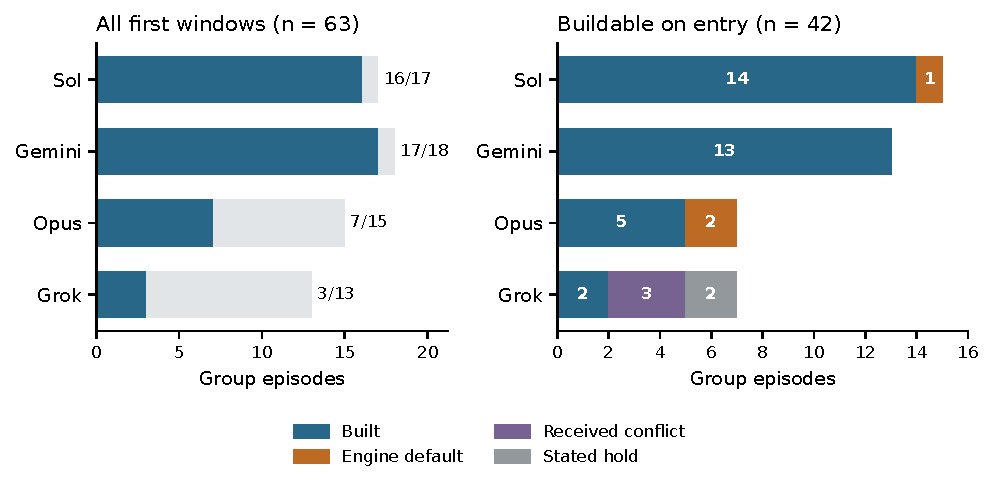
\includegraphics[width=\linewidth]{development.pdf}
\caption{First management after trade completion. Left: built groups over all acquired groups, including groups not buildable on entry. Right: all forty-two entry-buildable groups split by actual resolution. The eight non-builds comprise three defaults, three received END conflicts and two stated holds. A conflicting content request need not be executable as encoded. These conditional counts retain the distinct response policies; they do not measure willingness to invest.}
\label{fig:development}
\end{figure}
\begin{table}[t]
\centering\small
\begin{tabular}{lrrrrr}\toprule
Agent & Rejections & Some build & Same multiset & Changed multiset & Default\\\midrule
Sol & 29 & 25 & 20 & 5 & 4 \\
Gemini & 19 & 18 & 6 & 12 & 1 \\
Opus & 61 & 0 & 0 & 0 & 61 \\
Grok & 5 & 5 & 5 & 0 & 0 \\
\bottomrule\end{tabular}
\caption{Decisions with an uneven-intermediate-building rejection, followed through resolution. ``Some build'' means construction was applied in the same decision, not that the requested allocation or quantity was preserved. Opus's action-only recovery has already used the retry budget. Interleaving the identical purchases executes all 61 defaulted Opus multisets in exact-prefix tests; the original encodings were invalid.}
\label{tab:recovery}
\end{table}


All sixty-three trade-completed group episodes have an observed first management window. Forty-three receive construction in that window. Forty-two are buildable on entry, and thirty-four of those are developed during the window. Fifty-four become buildable at some point within it. The difference between entry and later legality matters because a player may first mortgage another deed or redeem the acquired property. Neither the 43/63 whole-path summary nor the 34/42 conditional summary measures willingness or general conversion skill. The first retains the consequences of acquisition and financing; the second describes responsiveness within an already available opportunity.

The eight entry-buildable groups without construction have different recorded explanations. Three end through engine defaults, three through received END actions that conflict with accompanying content, and two through consistent END records with stated reserve rationales. These are eight group episodes, not eight independent experiments. A conflict is not automatically a discarded executable build. One accompanying allocation is uneven as encoded, and another asks for finance. The other twenty-one groups are not entry-buildable, so they cannot simply be added to a tally of declined investments. Following the actual window separates groups that gain access from those that never do.

The construction audit explains one repeated execution failure in greater detail. An even final allocation can be illegal when submitted as consecutive grouped purchases, because intermediate states must also satisfy even building. All sixty-one Opus defaulted purchase multisets execute after interleaving the identical purchases. Sixty chains contain a refusal followed by an invalid action-only retry; G2 d129 has the invalid attempt before the refusal. The exhausted decision then applies END. Some plans contain hotels and require finishing construction in one group to return houses for another. The defect is execution order rather than the affordability or final allocation of those tested plans.

This mechanism is relevant to capability as deployed. The configured participant fails to realize an affordable allocation that it has represented in an attempted action. It does not identify how a different retry policy would change winning chances. Other participants also illustrate why recovery needs a finer definition than eventual legal construction. Among successful decisions following an uneven-building rejection, the original purchase multiset is preserved in 20/25 Sol, 6/18 Gemini and 5/5 Grok recoveries. The remaining successful recoveries change it. G2 d243's original seven-house target is legal after interleaving and leaves \$208; the actual retry and next decision buy six houses and leave \$358. In contrast, G14 d145--148 reaches the original eight-house target within the same global turn. Within-decision preservation and same-turn target attainment answer different questions.

Chosen restraint remains a substantive economic behavior. At G1 d426, Grok holds \$488 with one house on each yellow and applies a consistent END. Its corrected financing account reaches \$1,418. A legal extra Atlantic house would cost \$150, and subsequent liquidation would reach \$1,343. The \$75 difference is the purchase's resale loss. The hold preserves a measurable financing buffer without proving that it maximizes expected value. At G3 d176, Opus's valid action-only retry explicitly favors keeping \$204 over one \$150 house and a \$54 reserve; the record marks no fallback. A prior refusal therefore cannot, by itself, turn every later hold into an engine-authored default.

\subsection{Construction, realized income and inherited portfolios}

\begin{figure}[t]
\centering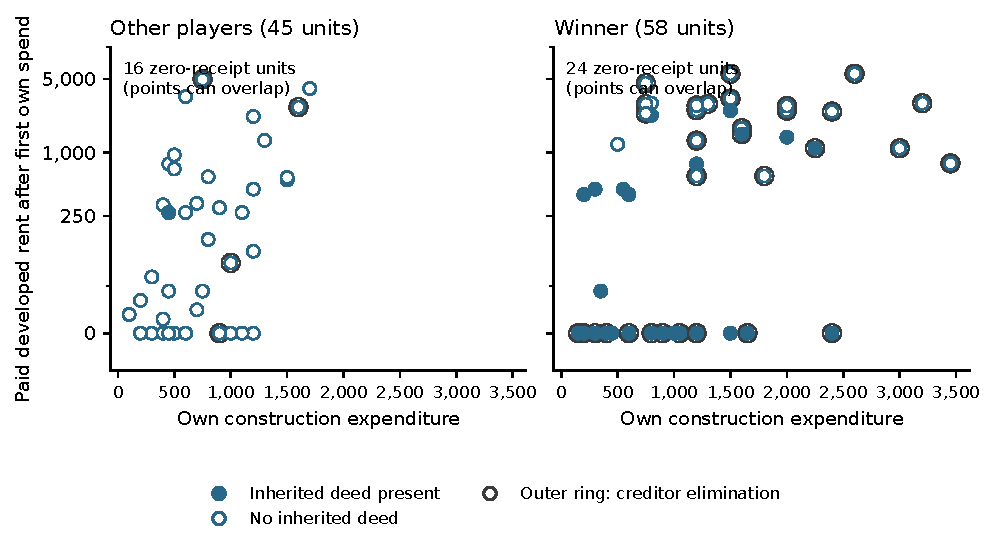
\includegraphics[width=\linewidth]{spending.pdf}
\caption{All 103 spending units, faceted by eventual winner status. Filled points contain an inherited deed at first own expenditure; outer rings indicate an elimination triggered by rent on that owner's group. The vertical axis is linear up to 250 and logarithmic above it. Forty units have zero paid developed receipts, with overlapping points on the baseline; twenty-six of them also trigger no creditor elimination. Receipts omit unpaid rent demands and are not net or incremental ROI. Winner status is a selected endpoint, not a treatment.}
\label{fig:spending}
\end{figure}

The 103 spending units incur \$103,450 in own construction expenditure. Whole-game paid developed rent to those units totals \$93,000, of which \$92,550 follows the owner's first own expenditure. The \$450 difference is G2 light-blue rent collected on inherited development before the winner's first own \$200 construction. Even the later window includes rent supported by inherited buildings. The totals describe expenditure and receipts on observed ownership paths; subtracting them does not yield net profit or construction's causal contribution.

Forty spending units collect no paid developed rent. Twenty-six of those also produce no creditor elimination on that group. These counts concern game/player/color units, whereas fifty-seven of sixty elimination events arise from rent on developed color properties. A large unpayable demand can end an opponent's game and transfer assets without appearing as a paid-rent receipt. Other zero-rent units retain assets, recover salvage, or face little remaining exposure. Denial and deterrence are possible sources of value but are not measured here. The data therefore support zero observed receipts, rather than forty failed investments.

Successive owners of G19's dark blues provide a concrete contrast. Opus spends \$1,200, receives \$175 in developed rent and later realizes \$600 in building sales. Gemini inherits the deeds, spends \$2,000 over its subsequent ownership, and receives \$1,400 in developed rent on a later Sol landing. The two units concern the same properties with different timing, financing and exposure. They show why an attractive group cannot guarantee receipts and why inherited ownership must remain visible. They do not isolate an owner effect. A recent \$1,200 construction step in the second trajectory must not be substituted for Gemini's \$2,000 cumulative own expenditure.

Winners account for fifty-eight spending units. Thirty-four contain at least one inherited deed at first own expenditure, while thirty first become complete through an estate. G3 brown, G6 light blue, G12 light blue and G14 green account for the distinction: inherited pieces are present, but later purchases or trades close the groups. A HOUSE\_BUILT-only definition would also miss G10's winner, which inherits four-house light blues and purchases \$150 in direct hotel conversions. The spending definition must include that case even though it records no own house purchase on the group.

Creditor inheritance is a major feature of the realized concentration of assets. The eventual winner is creditor in fifty-four of sixty eliminations, including thirty-five of forty nonterminal eliminations. Nineteen of twenty final eliminations name the winner as creditor; G13 ends with Luxury Tax owed to the bank. The nonterminal count is useful because it excludes estates received only when play has already ended. Under this implementation's declared variant, developed property can pass intact to a creditor. Productive assets accumulated by one player can consequently support another's later income and construction. The observed concentration is jointly determined by prior play, debts, movement and this rule. It is not a causal estimate of inheritance's advantage.

\subsection{Debt payment requires accessible finance}

\begin{figure}[t]
\centering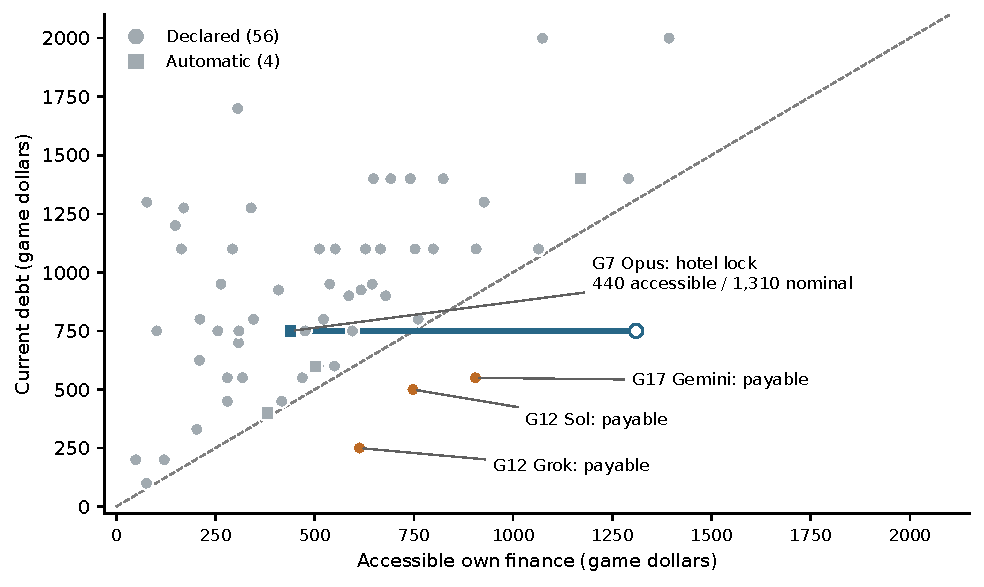
\includegraphics[width=\linewidth]{financing.pdf}
\caption{All sixty eliminations. Points above the diagonal owe more than accessible own finance. Fifty-six are insolvent even under a generous full bound, three have a tested legal payment route, and one is constrained by hotel liquidation. The G7 horizontal segment joins accessible \$440 to nominal \$1,310 against \$750 owed. Circles mark declarations and squares automatic eliminations. These are current-debt classifications without assumed assistance or an alternate-winner claim.}
\label{fig:financing}
\end{figure}

The elimination denominator comprises all sixty applied bankruptcies. Fifty-six follow declarations, and four occur automatically after mortgages exhaust the permitted continuation without covering the debt. In fifty-six cases, even the generous upper bound in Equation~\ref{eq:sol-upper} is below the current debt. Three current debts have engine-verified payment routes. The remaining case has enough nominal value but a binding hotel-liquidation restriction. Table~\ref{tab:sol-financing} states the local endpoints rather than inferring later survival.

\begin{table}[t]
\centering
\small
\begin{tabular}{llrrp{0.34\linewidth}}
\toprule
Case & Agent & Debt & Nominal upper & Local legal result \\
\midrule
G12 d190 & Sol & \$500 & \$748 & Payment route retains \$8. \\
G12 d249 & Grok & \$250 & \$613 & Five house sales pay; \$43 remains. \\
G17 d234 & Gemini & \$550 & \$905 & Sales and two mortgages pay; \$155 left. \\
G7 d339 & Opus & \$750 & \$1,310 & Only \$440 is accessible; hotel sale is locked. \\
\bottomrule
\end{tabular}
\caption{Four eliminations not ruled out by the nominal upper bound. Payment routes need not realize the entire upper bound. The other fifty-six eliminations cannot cover the current debt even under that bound. All sixty cases exclude assumed assistance from another player.}
\label{tab:sol-financing}
\end{table}

The payable cases do not share a single reasoning mechanism. At G12 d190, Sol's stated \$408 maximum omits red collateral unlocked by selling houses. At G17 d234, Gemini's \$530 account understates a route involving sales and Baltic and Park Place mortgages. G12 d249 instead contains a sharp action/explanation disagreement. Its accompanying content requests house sales, and its final provider and applied private explanations recommend survival, while the received tool declares bankruptcy. Five legal one-house sales already cover the debt without a mortgage. The applied elimination is avoidable at that local endpoint, but the record does not identify an intention to surrender or justify calling all three cases deliberate choices.

Successful liquidation supplies a necessary contrast. G18 d428 sells development and mortgages red collateral, pays \$750 and retains \$69. G20 d327--336 starts with \$49, realizes \$700 in salvage and \$665 in mortgages, pays \$1,400, and retains \$14 using the actual stock constraints. These paths exhibit staged financing and preservation of continued participation. At G16 d602, a twenty-three-step legal liquidation reaches \$1,393 against \$2,000 owed, so even extensive correct execution cannot pay. The applied private note already reports the correct total; a generated research label instead gives \$1,233 by omitting \$160 of unlocked light-blue collateral. Legal-sequence checking corrects the analyst as well as the agent.

Finite stock creates a different limit. Nine games reach zero bank houses in initial decision payloads, but an empty bank does not establish an agent's desire for a blocked project. At G7 d339, Opus has pinks at four houses, four houses and a hotel. Too few bank houses prevent downgrading the hotel, and even-selling prevents selling a lower sibling first. Its \$390 cash and Oriental mortgage yield only \$440 against \$750, despite \$1,310 nominal value. Exhausting both permitted mortgage orders leaves the sale menu empty. This establishes a genuine current-debt lock. Earlier opportunities to convert hotels and release houses belong to different states and cannot be carried forward as an escape from that debt.

Other scarcity cases allow costly adjustment. At G12 d312, a direct Illinois hotel is blocked with reds at 3/3/4 and no bank houses, yet a longer legal restructuring reaches it with \$26 and four bank houses remaining. That route changes other development and reserves. At G5 d300, a legal \$100 pink hotel would release four houses, but retaining the houses does not by itself establish that a funded rival project was denied. These cases distinguish immediate restrictions, reachable reallocation and expressed demand. Economic planning in this cohort consists of choosing among such consequential allocations, sometimes executing them successfully, sometimes preserving reserves, and sometimes losing an accessible action through the response process. The accompanying bargaining statements require a separate reconstruction of what counterparties saw and how they responded.
